\section{Использование диаметра области}
\label{compact:diameter}

\paragraph{Известный диаметр.}
Совместная огибающая допускает точное ограничение по диаметру.
Диаметр можно ограничить сверху или задать точно; сама область
при этом может меняться.

\begin{theorem}[Совместная огибающая при известном диаметре]
\label{jointdiam:main}
Пусть выполнено \eqref{boundarygap:assumptions} и $D>0$.
Для $g,P>0$ положим
\begin{equation}\label{jointdiam:definition}
 \begin{gathered}
 h=\min\{g,P^2/m,PD\},\qquad
 \rho_-=h^2/P^2,\qquad \rho_+=\min\{h/m,D^2\},\\
 \mathcal J_D(g,P)=\max_{\rho_-\le\rho\le\rho_+}V(h,\rho).
 \end{gathered}
\end{equation}
Положим $\mathcal J_D(g,0)=\mathcal J_D(0,P)=0$. Тогда
\[
 G(x)\le g,\quad \|\nabla f(x)\|\le P,\quad
 \operatorname{diam}Q\le D
 \quad\Longrightarrow\quad
 \delta(x)\le\mathcal J_D(g,P).
\]
Оценка точна для этих трёх верхних границ. Тот же супремум
получается при $\operatorname{diam}Q=D$. К нему приближаются
гладкие функции на окрестностях треугольников с непустой
внутренностью в $\mathbb R^2$.

При точно заданных положительных значениях $G(x)=g$ и
$\|\nabla f(x)\|=P$ класс непуст в точности при $g\le PD$.
Если это условие выполнено, супремум снова равен
$\mathcal J_D(g,P)$ как при диаметре не более $D$,
так и при диаметре ровно $D$.
\end{theorem}

При $H_1=0$ положим
$\beta=(H_0^2-2mH_0-m^2)/(4H_0)$. Тогда
\begin{equation}\label{jointdiam:constant}
 \mathcal J_D(g,P)=
 \begin{cases}
 h+\beta\rho_+,&\beta\ge0,\\
 h+\beta\rho_-,&\beta<0.
 \end{cases}
\end{equation}
Например, при $m=1$, $H_0=4$, $H_1=0$, $g=1$, $P=2$ и
$D=3/5$ получаем
\[
 \beta=7/16,\qquad
 \mathcal J_D(1,2)=463/400<23/16=\mathcal J(1,2).
\]
Оба наблюдения могут быть точными, поскольку $g=1<6/5=PD$.
При $H_1>0$ и $\mathcal S(h)\le0$ монотонность по радиусу даёт
\begin{equation}\label{jointdiam:ordinary}
 \mathcal J_D(g,P)=V(h,\rho_-)
       \le h+\rho_-\mathcal S(h)\le h.
\end{equation}
Поэтому в режиме обычного зазора по-прежнему достаточно одного
уравнения переключения или указанной алгебраической верхней оценки.

\begin{corollary}[Огибающая по норме при известном диаметре]
\label{jointdiam:norm}
Для $P>0$ положим $r_D=\min\{D,P/m\}$ и
$q=\max\{P-mD,0\}$. Точная оценка только по норме при
диаметре не более $D$ равна
\begin{equation}\label{jointdiam:norm-formula}
 \mathcal E_D(P)=\mathcal J_D(PD,P)
       =A(P,r_D)=\mathcal E_q(P).
\end{equation}
Она остаётся точной при одновременных равенствах
$\|\nabla f(x)\|=P$ и $\operatorname{diam}Q=D$.
Положим $\mathcal E_D(0)=0$.
Если $H_1=0$ и $P\ge mD$, то
\begin{equation}\label{jointdiam:norm-constant}
 \mathcal E_D(P)=PD+\beta D^2.
\end{equation}
При фиксированном $D$ это аффинная функция $P$.
\end{corollary}

\begin{figure}[htbp]
\centering
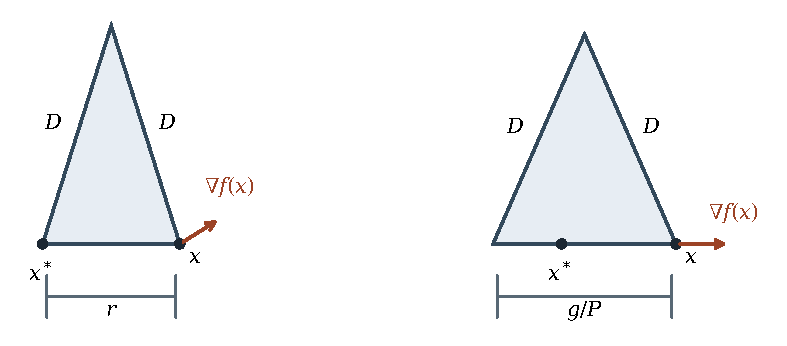
\includegraphics[width=0.9\linewidth]{figures/diameter_geometry.pdf}
\caption{Конструкции точности для допустимых точных наблюдений. Слева: активен зазор, $g\le P^2/m$. Справа: активна норма, $P^2/m<g\le PD$. Обе наклонные стороны имеют длину $D$.}
\label{jointdiam:geometry}
\end{figure}

\paragraph{Доказательство теоремы~\ref{jointdiam:main}.}
Из определения следует $0<\rho_-\le\rho_+$; непрерывность $V$
обеспечивает существование максимума. Для неоптимального источника
обозначим $r=\|x-x^*\|$, а через $p$ его конечную радиальную
производную. Сдвинутое RSI и условие минимума на области дают
$mr\le p\le P$; кроме того, $pr\le G(x)\le g$ и $r\le D$.
Следовательно,
\[
 pr\le\min\{g,P^2/m,PD\}=h,\qquad
 r\le R:=\min\{\sqrt{h/m},D\}.
\]
Положим $r_0=h/P\le R$. Радиальная огибающая $A(P,r)$ из
\eqref{joint:radial-identity} строго возрастает по $r$.
При $r\le r_0$ она ограничивает ошибку величиной
$A(P,r_0)=V(h,r_0^2)$. При $r\ge r_0$ верхние границы $h/r$
для конечной и $h/r-mr$ для начальной производной дают оценку
$V(h,r^2)$. Тем самым доказано \eqref{jointdiam:definition}.
Нулевой зазор или нулевая норма в силу сдвинутого RSI означают
нулевую ошибку. Нулевая оценка достигается в точке минимума
квадратичной функции на треугольнике диаметра $D$.

Для доказательства точности выберем максимизирующий радиус
$\rho$ и положим
\[
 r=\sqrt\rho,\quad p=h/r,\quad q=p-mr,\quad
 c=\sqrt{P^2-p^2},\quad a_D=\sqrt{D^2-r^2/4}.
\]
Скалярная конструкция из леммы~\ref{compact:radial}
даёт гладкие функции $u_j$ на окрестностях $[0,r]$ с условиями
\[
 \begin{gathered}
 u_j(0)=0,\quad u_j'(0)=q,\quad u_j'(r)=p,\quad
 u_j'(s)-q\ge ms,\\
 |u_j''(s)|\le H_0+H_1u_j(s),\qquad
 u_j(r)\longrightarrow V(h,\rho).
 \end{gathered}
\]
Определим
\[
 Q=\operatorname{conv}\{(0,0),(r,0),(r/2,a_D)\},\qquad
 f_j(s,y)=u_j(s)+cy+my^2/2.
\]
Две боковые стороны имеют длину $D$, а основание имеет длину
$r\le D$. Поэтому диаметр $Q$ равен ровно $D$, и внутренность
непуста. В его точках $0\le s\le r$ и $y\ge0$.
Единственная точка минимума есть $(0,0)$; всюду на $Q$
\[
 \langle\nabla f_j(s,y)-\nabla f_j(0,0),(s,y)\rangle
       =(u_j'(s)-q)s+my^2\ge m(s^2+y^2),
\]
\[
 \|\nabla^2f_j(s,y)\|
       =\max\{|u_j''(s)|,m\}
       \le H_0+H_1u_j(s)\le H_0+H_1f_j(s,y).
\]
В точке $(r,0)$ градиент равен $(p,c)$ и имеет норму $P$.
Его скалярное произведение с точками области минимально в
$(0,0)$, так что полный зазор равен $pr=h\le g$.
Ошибка источника стремится к $\mathcal J_D(g,P)$.
Это доказывает точность для верхних границ, в том числе при
точно заданном диаметре.

Для точных положительных наблюдений условие $g\le PD$
необходимо, поскольку
$G(x)\le\|\nabla f(x)\|\operatorname{diam}Q$.
Если также $g\le P^2/m$, то $h=g$, и предыдущая конструкция
уже задаёт оба наблюдения точно. Если $P^2/m<g\le PD$, положим
\[
 r=P/m,\qquad a=g/P-r,\qquad \ell=r+a=g/P\le D.
\]
Возьмём гладкие скалярные профили на $[0,r]$ с нулевой начальной
производной и конечной производной $P$, приближающие $\mathcal E(P)$.
Сглаживание затрагивает только внутреннее переключение,
поэтому около нуля они совпадают с
\[
 u_+(s)=
 \begin{cases}
 (H_0/H_1)\{\cosh(\sqrt{H_1}s)-1\},&H_1>0,\\
 H_0s^2/2,&H_1=0.
 \end{cases}
\]
Продолжим их на $[-a,0]$ этой чётной функцией. На добавленном
отрезке $|u_+''|=H_0+H_1u_+$ и $u_+'(s)s\ge ms^2$.
Обозначим продолжение через $u_j$. На треугольнике
\[
 Q=\operatorname{conv}\left\{(-a,0),(r,0),
       \left((r-a)/2,\sqrt{D^2-\ell^2/4}\right)\right\}
\]
положим $f_j(s,y)=u_j(s)+my^2/2$.
Снова $\operatorname{diam}Q=D$, точка минимума есть $(0,0)$,
а сдвинутое RSI и ограничение Гессиана выполнены на всём $Q$.
Градиент источника равен $(P,0)$; линейный оракул выбирает
$(-a,0)$ и даёт зазор $P\ell=g$. Ошибка стремится к
$\mathcal E(P)=\mathcal J_D(g,P)$.
Все функции гладкие на окрестностях своих треугольников.

Формула \eqref{jointdiam:constant} получается максимизацией
аффинной по радиусу функции $h+\beta\rho$.
Формула \eqref{jointdiam:ordinary} следует из
следствия~\ref{gapregime:radius-monotone} при $\rho_-$.
Для следствия~\ref{jointdiam:norm} граница зазора $PD$
следует из ограничений на норму и диаметр.
В $\mathcal J_D(PD,P)$ отрезок радиусов состоит из одной
точки $r_D^2$, а начальная производная равна
$P-mr_D=\max\{P-mD,0\}=q$.
Радиальное тождество и предложение~\ref{joint:fixed-slope}
дают \eqref{jointdiam:norm-formula}; формула радиальной
огибающей при постоянной кривизне даёт
\eqref{jointdiam:norm-constant}.

\paragraph{Полный зазор при известном диаметре.}
Для $D>0$ определим
\begin{equation}\label{compact:gap-diameter}
 \mathcal B_D(g)=
 \max_{0\le\rho\le\min\{g/m,D^2\}}V(g,\rho),\qquad
 \mathcal B_D(0)=0.
\end{equation}
При $\operatorname{diam}Q\le D$ имеем
$\delta(x)\le\mathcal B_D(G(x))\le\mathcal B(G(x))$.
Это точный супремум при фиксированном полном зазоре и границе
диаметра. Функция $\mathcal B_D$ непрерывна и удовлетворяет
\eqref{boundarygap:growth}.

Действительно, радиальная верхняя оценка использует $r\le D$,
а гладкие примеры на $[0,r]$ из леммы~\ref{compact:radial}
приближают все значения с $r\le D$.
Предел $\rho\downarrow0$ обеспечивают те же линейно-квадратичные
примеры, что в доказательстве теоремы~\ref{boundarygap:main}.
Замена $\rho=z\min\{g/m,D^2\}$, $z\in[0,1]$, доказывает
непрерывность; добавление линейного слагаемого доказывает рост,
не меняя длину отрезка.

При $H_1=0$
\[
 \mathcal B_D(g)=g+\max\{0,\beta\}\min\{g/m,D^2\}.
\]
При $H_1>0$, $g>0$ имеем точный критерий
\[
 \mathcal B_D(g)=g\quad\Longleftrightarrow\quad\mathcal S(g)\le0.
\]
При неположительном знаке достаточно
$g\le\mathcal B_D(g)\le\mathcal B(g)=g$.
При положительном знаке первая вариация
\eqref{gapregime:variation} превышает $g$ при сколь угодно
малых положительных радиусах, удовлетворяющих также $\rho\le D^2$.
Для скалярного вычисления применяется предложение~\ref{boundarygap:budget}
на укороченном отрезке с $\ell=g$.
